\chapter{\ifproject%
\ifenglish Experimentation and Results\else การทดลองและผลลัพธ์\fi
\else%
\ifenglish System Evaluation\else การประเมินระบบ\fi
\fi}

% ในบทนี้จะทดสอบเกี่ยวกับการทำงานในฟังก์ชันหลักๆ
ในบทนี้จะทดสอบระบบการยืนยันตัวตนด้วยการใช้ภาพใบหน้าบุคคล ซึ่งมีการเก็บข้อมูลรูปภาพใบหน้าบุคคล เพื่อทำการทดลองเป็นเวลา 5 วัน เพื่อดูผลการทดลองในด้านต่าง ๆ ของแต่ละวัน ได้แก่ 
การออกแบบอุปกรณ์ตรวจจับภาพใบหน้าบุคคล และหน้าแสดงผลทางหน้าจอ ความแม่นยำในการตรวจจับรูปภาพใบหน้าบุคคล ความแม่นยำของการระบุตัวตนด้วยรูปภาพใบหน้าบุคคล 
เวลาในการประมวลผลรูปภาพใบหน้าบุคคลตลอดถึงการแสดงผล 
และความพึงพอใจของผู้ทดลองต่อระบบ

\section{การออกแบบอุปกรณ์ตรวจจับภาพใบหน้าบุคคล และหน้าแสดงผลทางหน้าจอ (GUI)}

\subsection{รูปอุปกรณ์ที่ใช้ในการตรวจจับภาพใบหน้าและรับคำสั่งยืนยัน}

\begin{figure}[!ht]
  \begin{center}
    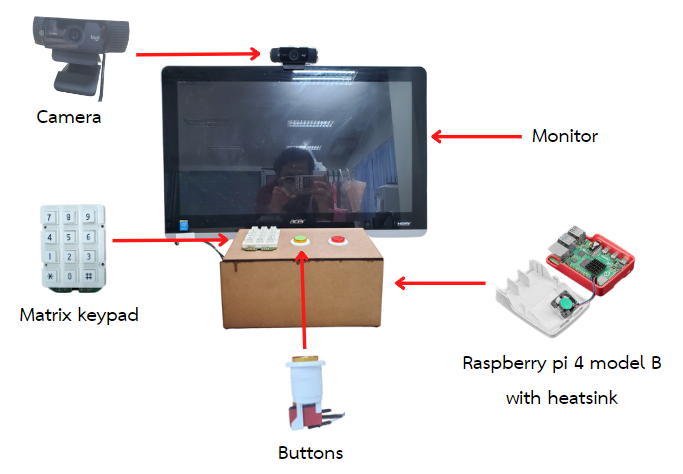
\includegraphics[scale=.6]{pic/overall_module.png}
    \caption[อุปกรณ์ตรวจจับใบหน้า แสดงผลและรับผล]{อุปกรณ์ตรวจจับใบหน้า แสดงผลและรับผล}
    \label{fig:module_pi}
  \end{center}
\end{figure}


\begin{figure}[!ht]
  \begin{center}
    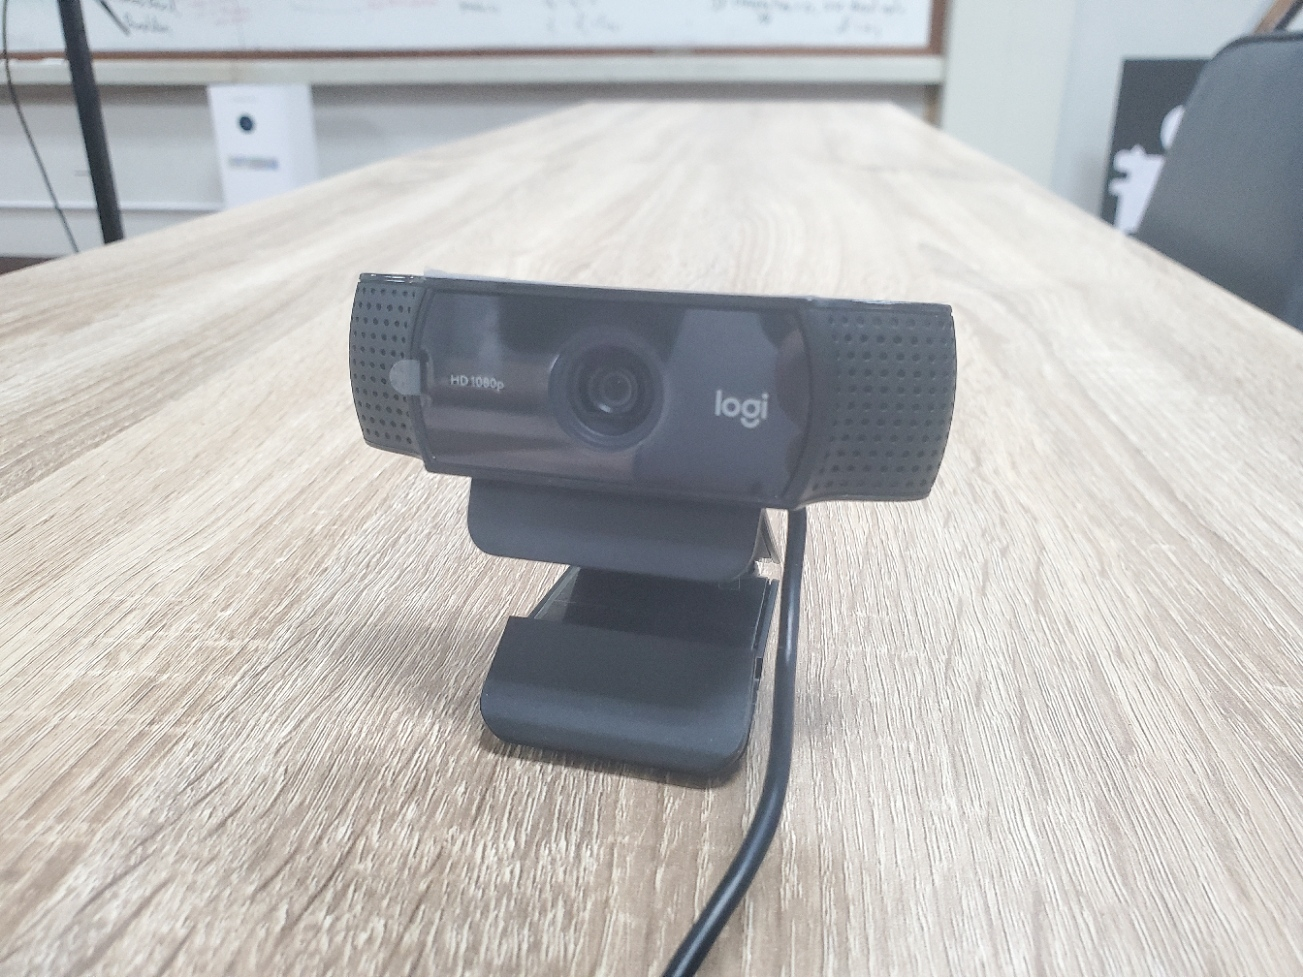
\includegraphics[scale=.15]{pic/camera.jpg}
    \caption[กล้องที่ใช้ในการตรวจจับใบหน้าบุคคล]{กล้องที่ใช้ในการตรวจจับใบหน้าบุคคล}
    \label{fig:camera_logi}
  \end{center}
\end{figure}



\begin{figure}[!ht]
  \begin{center}
    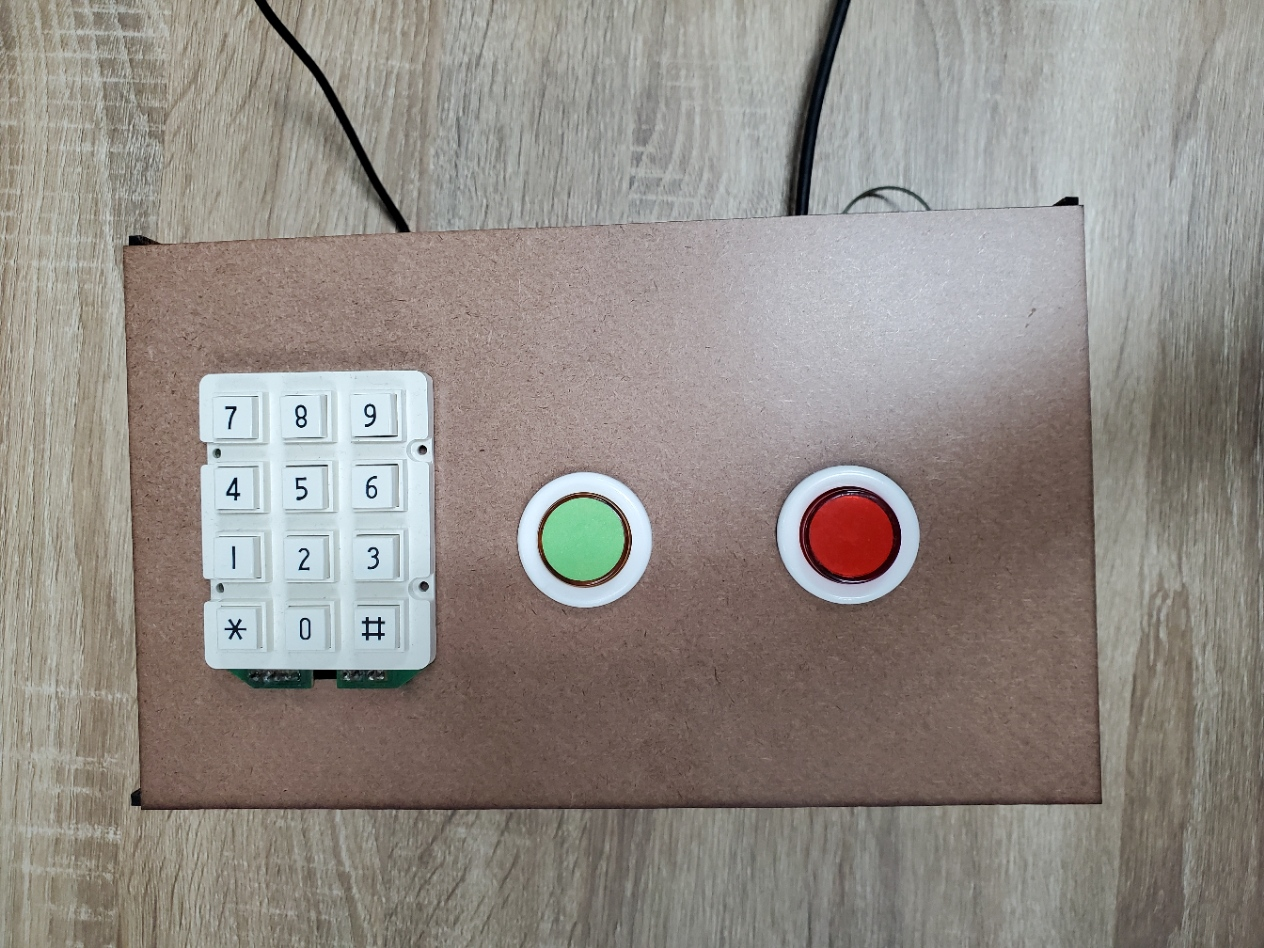
\includegraphics[scale=.17]{pic/rpi_top.jpg}
    \caption[ปุ่มกดยืนยันความถูกต้องของการระบุตัวตน]{ปุ่มกดยืนยันความถูกต้องของการระบุตัวตน}
    \label{fig:button_module}
  \end{center}
\end{figure}

\begin{figure}[!ht]
  \begin{center}
    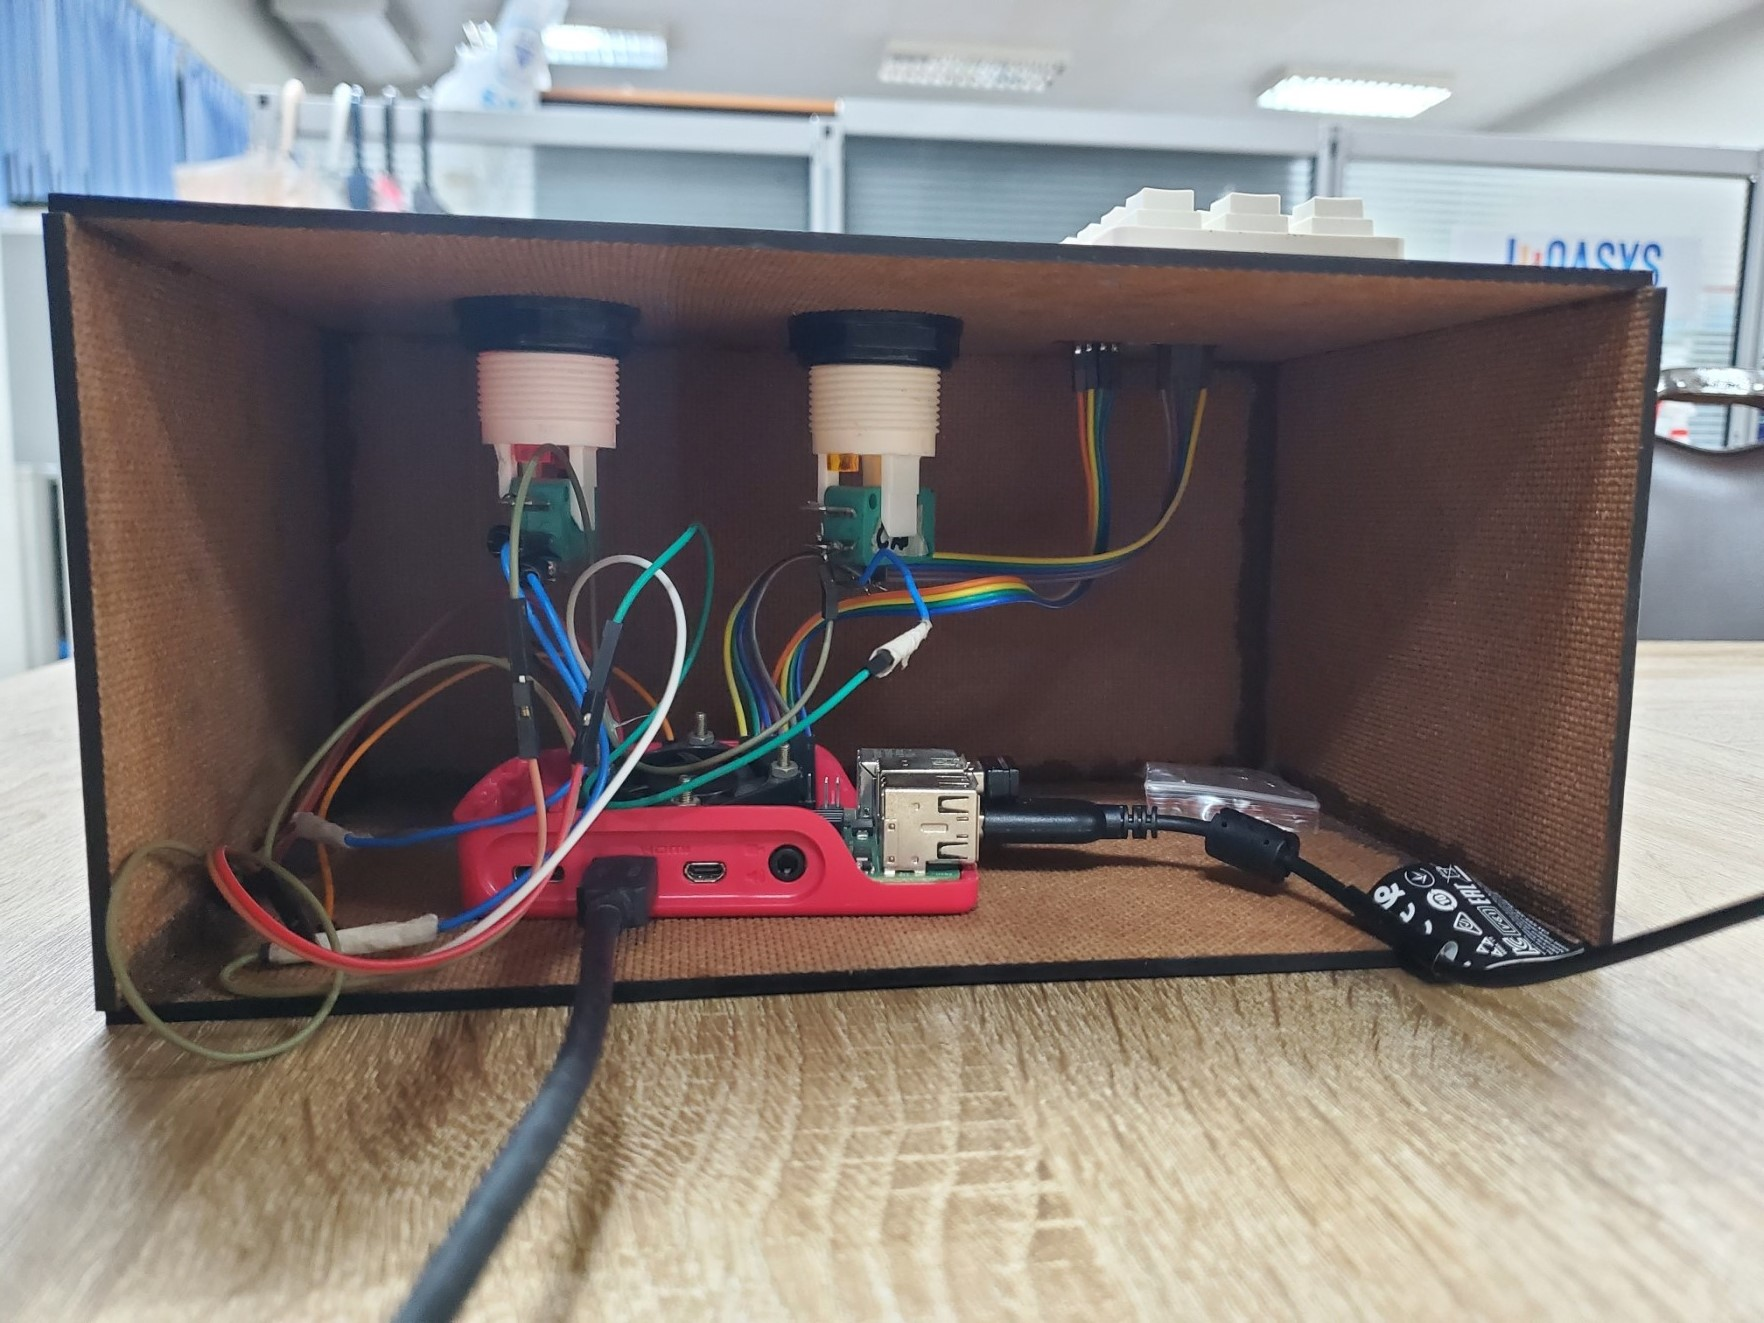
\includegraphics[scale=.17]{pic/rpi_back.jpg}
    \caption[ภายในมอดูลการตรวจจับใบหน้า และแสดงผล]{ภายในมอดูลการตรวจจับใบหน้า และแสดงผล}
    \label{fig:inside_module}
  \end{center}
\end{figure}

\begin{figure}[!ht]
  \begin{center}
    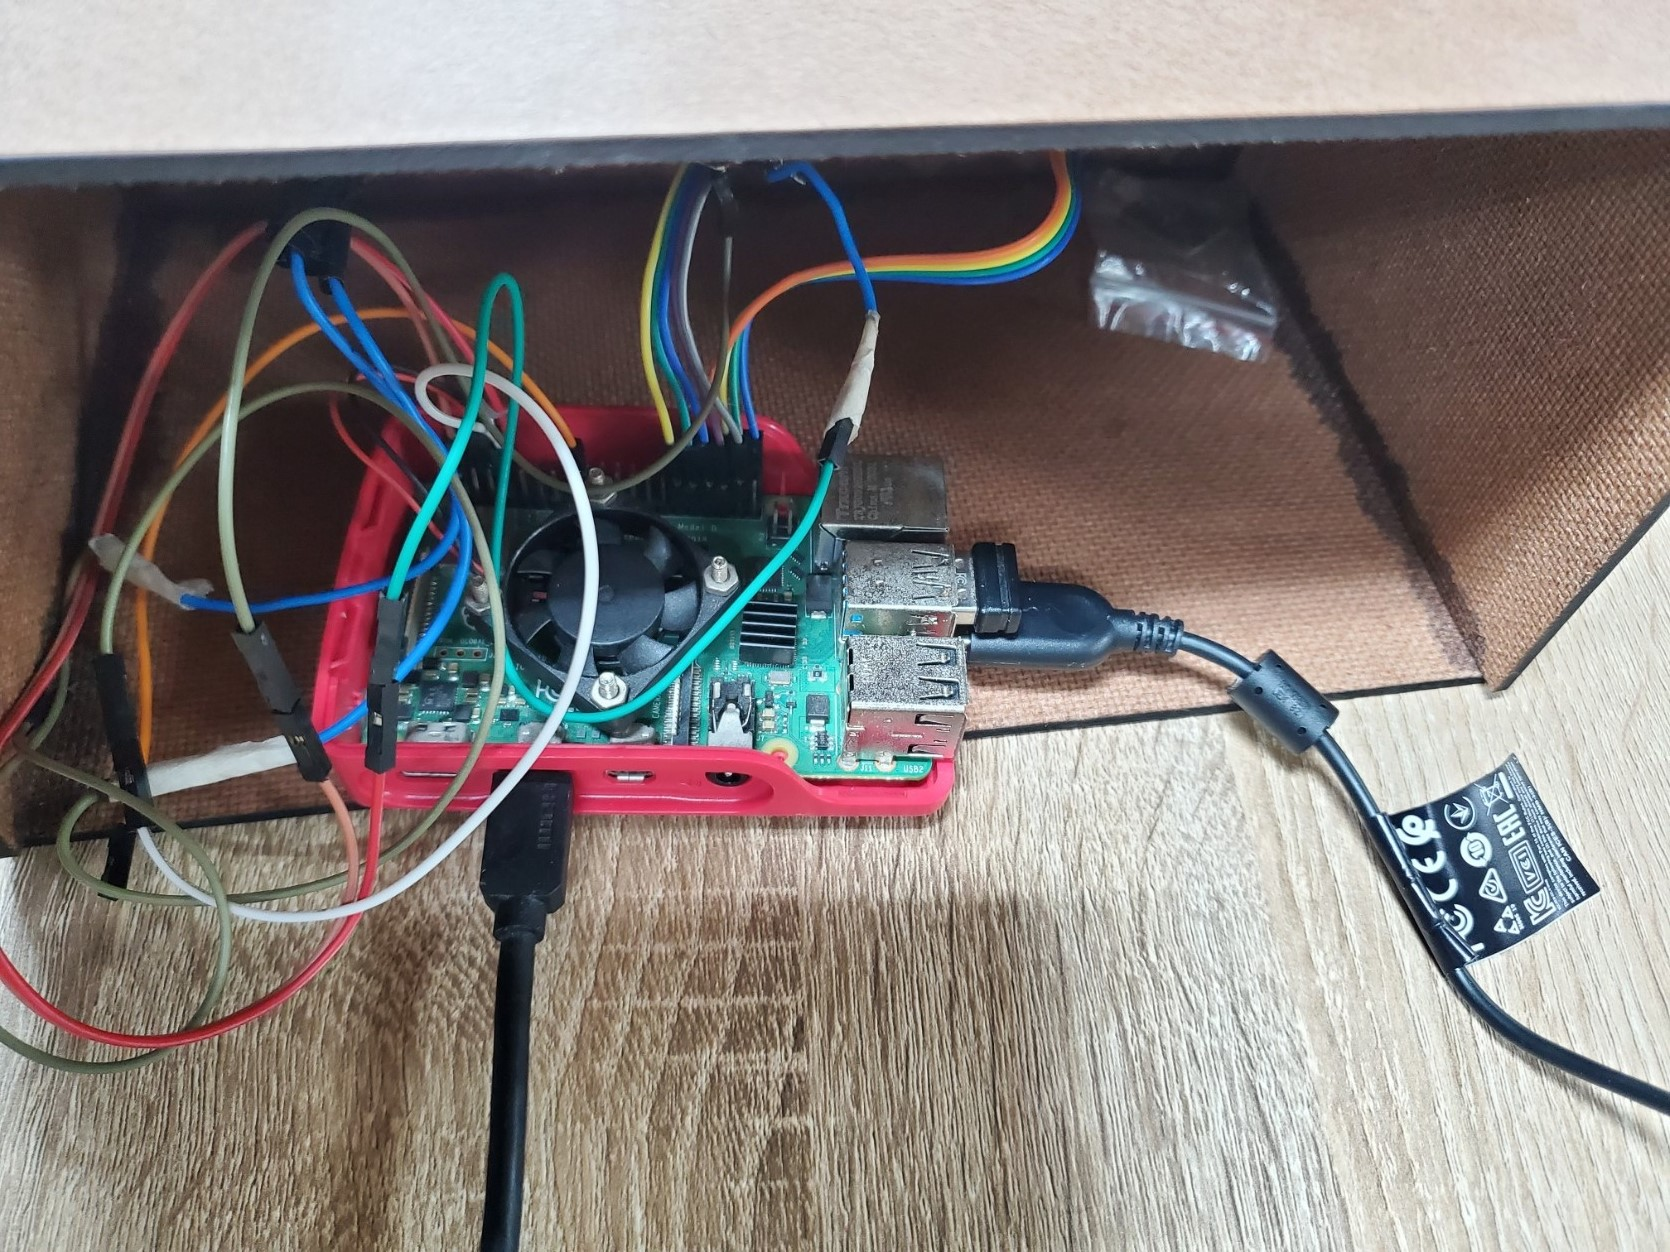
\includegraphics[scale=.17]{pic/rpi.jpg}
    \caption[การเชื่อมต่อ Raspberry Pi]{การเชื่อมต่อ Raspberry Pi}
    \label{fig:rpi_module}
  \end{center}
\end{figure}

\newpage
\subsection{รูปภาพการแสดงผลบนหน้าจอ}

\begin{figure}[!ht]
    \begin{center}
      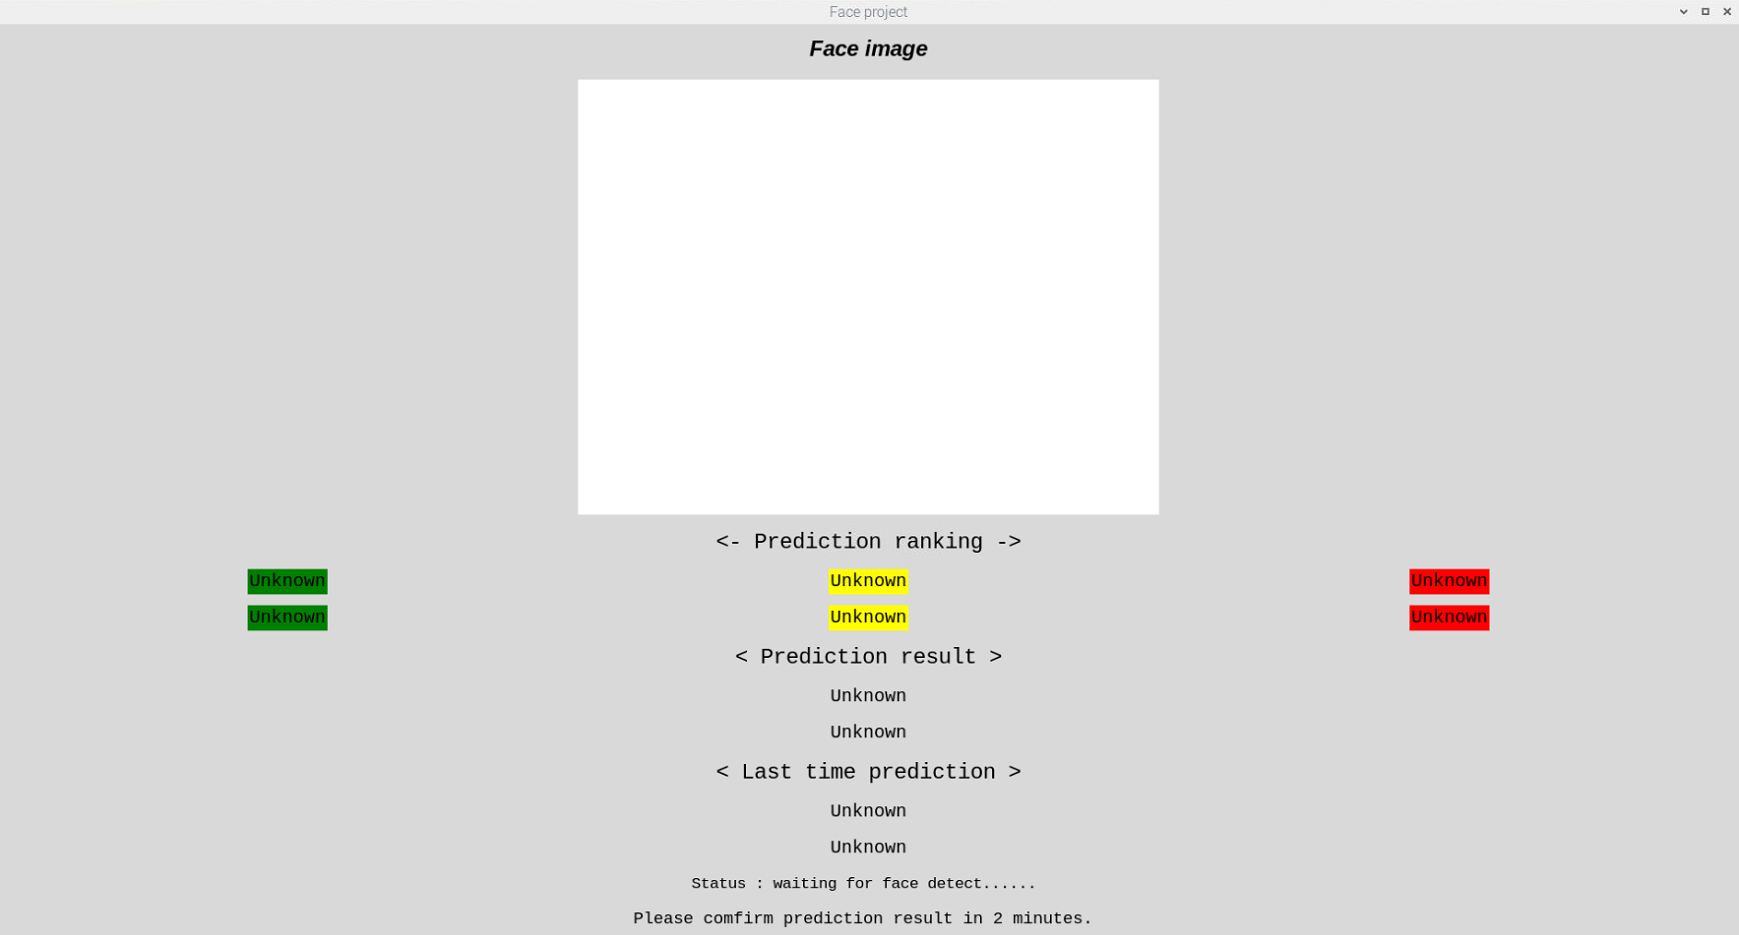
\includegraphics[scale=.25]{pic/main_page.png}
      \caption[หน้า GUI เมื่อโปรแกรมเริ่มทำงาน]{หน้า GUI เมื่อโปรแกรมเริ่มทำงาน}
      \label{fig:main_page}
    \end{center}
\end{figure}



\begin{figure}[!ht]
    \begin{center}
      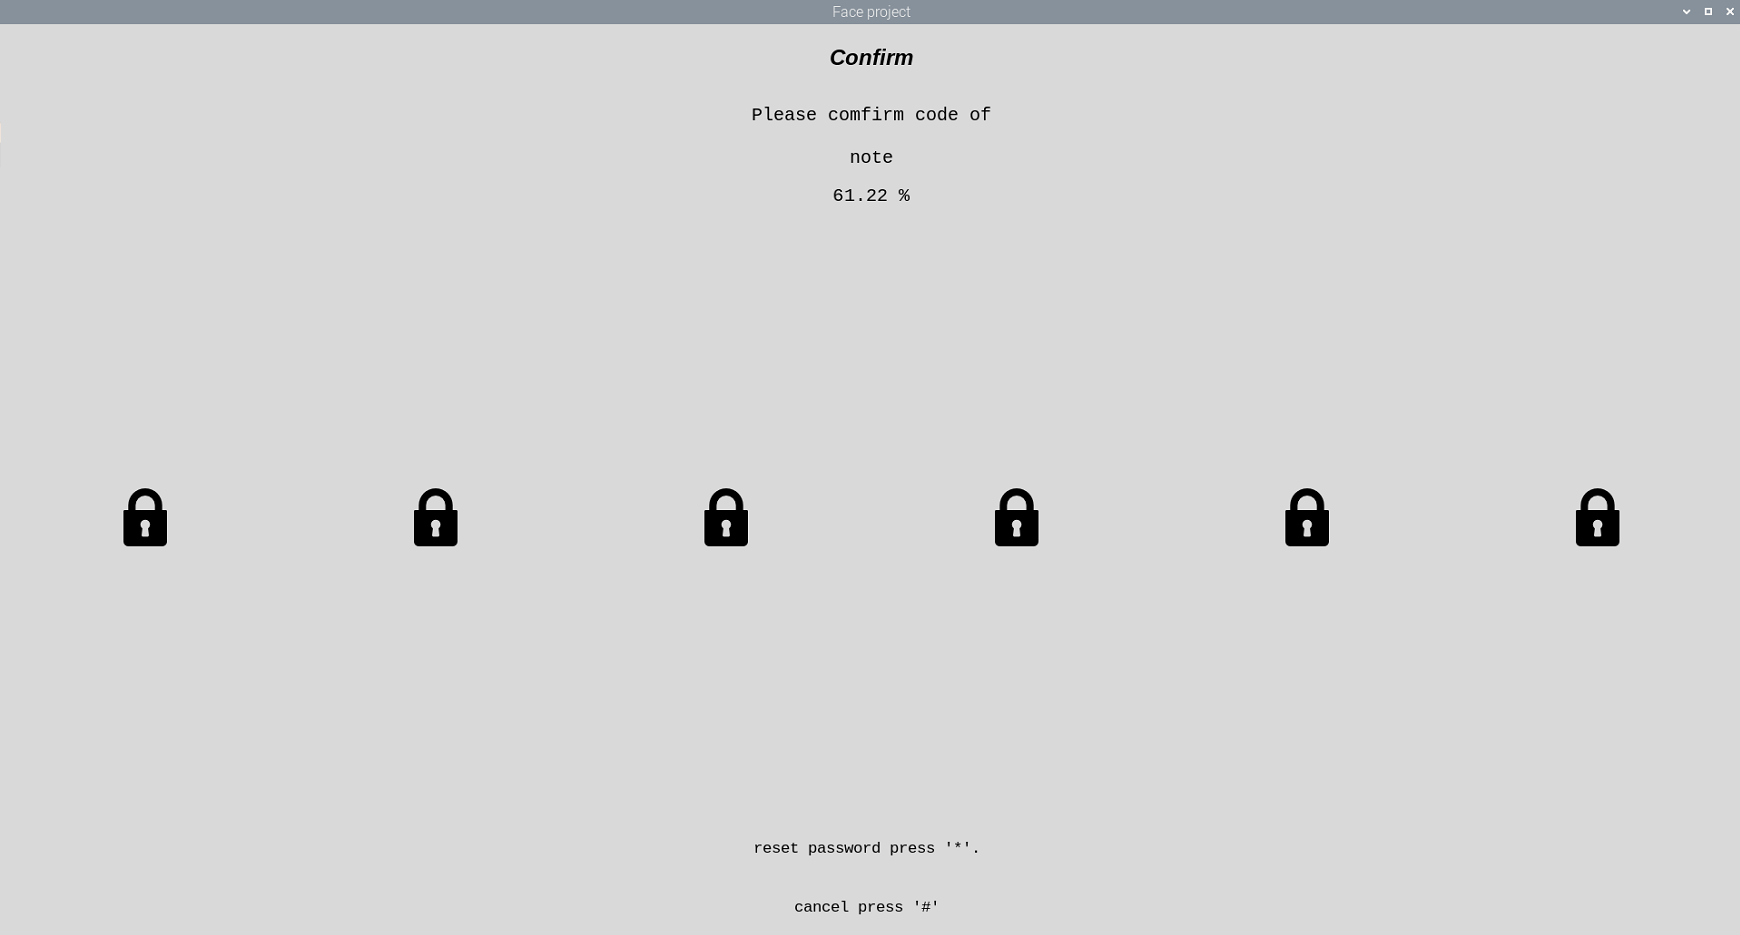
\includegraphics[scale=.25]{pic/comfirm_page.png}
      \caption[หน้า GUI เมื่อผลลัพธ์การระบุตัวตนผิด]{หน้า GUI เมื่อผลลัพธ์การระบุตัวตนผิด}
      \label{fig:com_page}
    \end{center}
\end{figure}


\begin{figure}[!ht]
  \begin{center}
    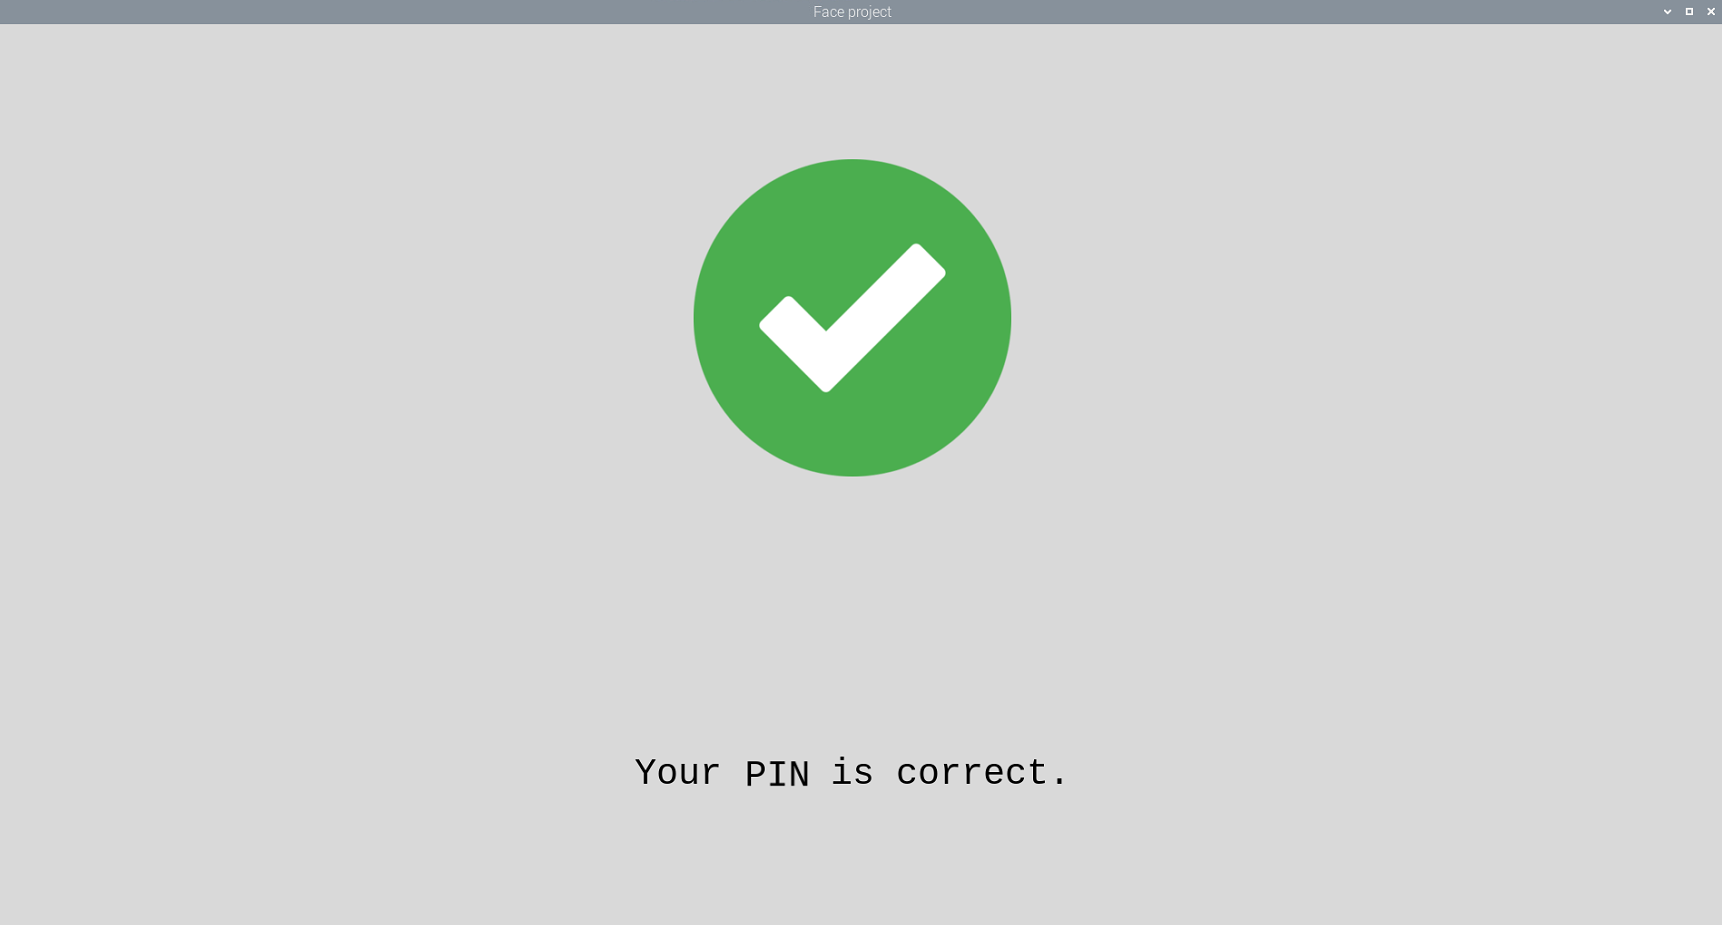
\includegraphics[scale=.25]{pic/pin_correct.png}
    \caption[หน้า GUI เมื่อผลลัพธ์รหัสยืนยันตัวตนถูกต้อง]{หน้า GUI เมื่อผลลัพธ์รหัสยืนยันตัวตนถูกต้อง}
    \label{fig:pin_correct}
  \end{center}
\end{figure}


\begin{figure}[!ht]
  \begin{center}
    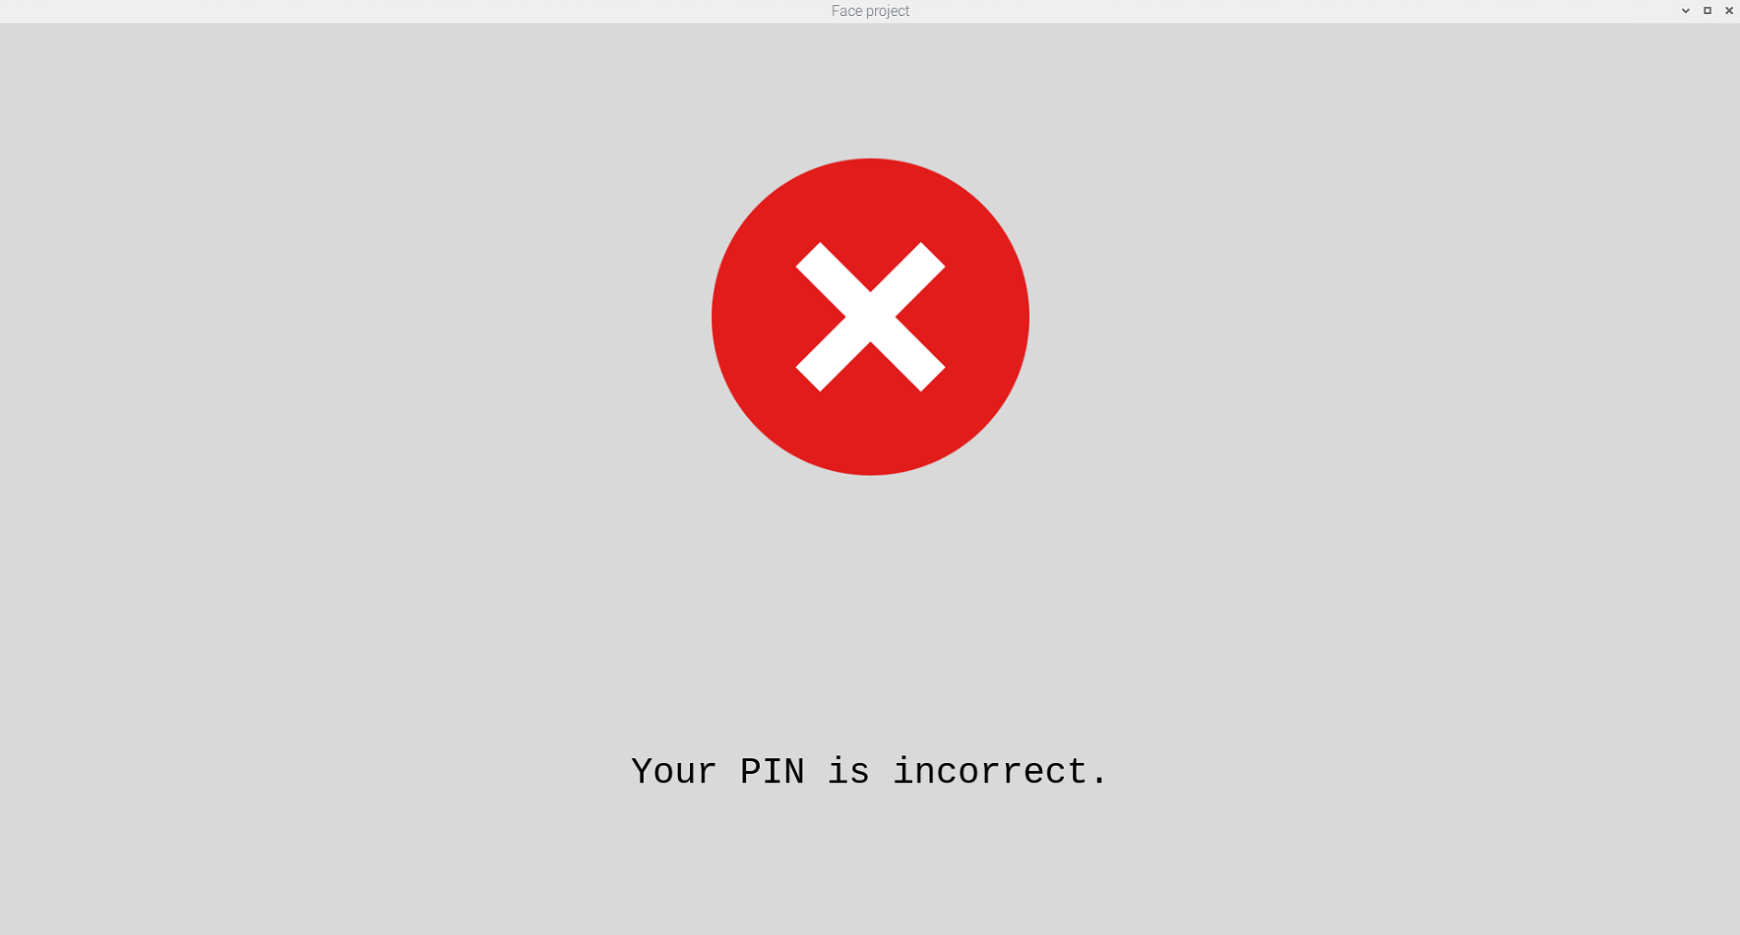
\includegraphics[scale=.25]{pic/pin_incorrect.png}
    \caption[หน้า GUI เมื่อผลลัพธ์รหัสยืนยันตัวตนไม่ถูกต้อง]{หน้า GUI เมื่อผลลัพธ์รหัสยืนยันตัวตนไม่ถูกต้อง}
    \label{fig:pin_incorrect}
  \end{center}
\end{figure}

\newpage

\section{ความแม่นยำของการตรวจจับใบหน้า}
การทดสอบนี้จะเป็นการทดสอบเพื่อวัดผลความแม่นยำในการตรวจจับภาพใบหน้าบุคคล โดยมีรูปภาพใบหน้าบุคคลจำนวน 50 รูป และรูปภาพสัตว์จำนวน 50 รูป 
ทำการทดลองกับแบบจำลองการตรวจจับใบหน้าบุคคลได้ผลลัพธ์ดังกราฟด้านล่าง

\begin{figure}[!ht]
  \begin{center}
    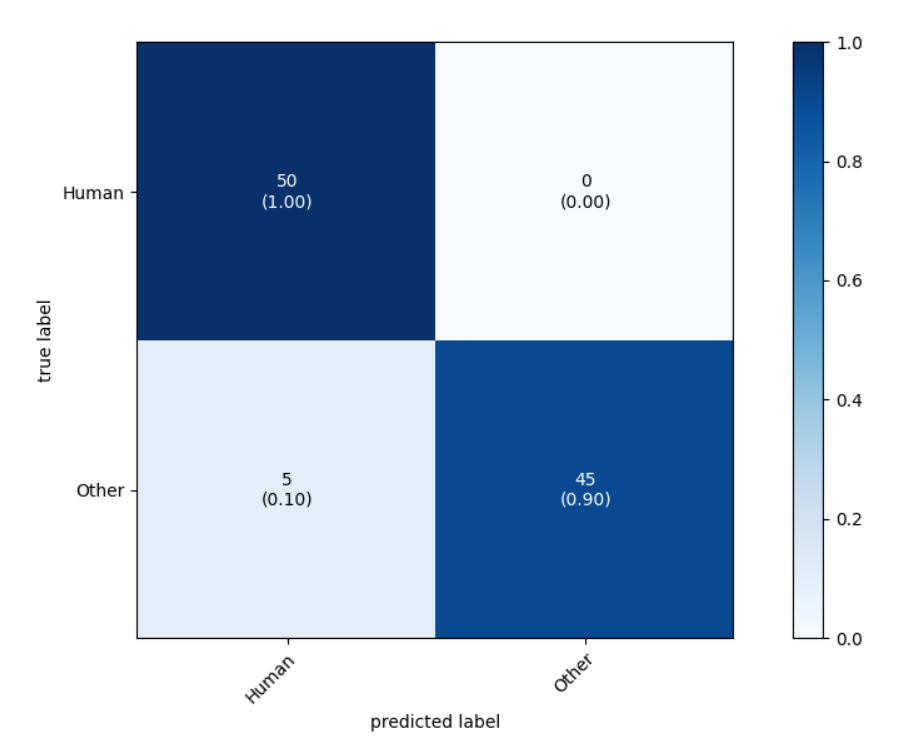
\includegraphics[scale=.55]{pic/face_result.png}
    \caption[กราฟแสดงความแม่นยำของการตรวจจับใบหน้า]{กราฟแสดงความแม่นยำของการตรวจจับใบหน้า}
    \label{fig:acc_graph}
  \end{center}
\end{figure}
\newpage
\indent จากกราฟจะสามารถคำนวนความแม่นยำได้ดังสูตร 
\begin{equation}\label{eq:Precision}
Precision=\frac{True Positive}{True Positive + False Positive}=\frac{50}{50+0} = 1.0
\end{equation}

\begin{equation}\label{eq:Accuracy}
Accuracy=\frac{True Positive + True Nagative}{Positive + Negative}=\frac{50+45}{50+50} = 0.95
\end{equation}

\begin{equation}\label{eq:F1Score}
F1 Score=\frac{2\cdot True Positive}{2\cdot True Positive + False Positive + False Negative}=\frac{2\cdot 50}{2\cdot 50+0+5} = 0.9524
\end{equation}

\section{ความแม่นยำของการระบุตัวตนด้วยใบหน้าในแต่ละวัน}
การทดสอบนี้จะเป็นการทดสอบเพื่อวัดผลความแม่นยำในการระบุตัวตน โดยความแม่นยำจะมีแนวโน้มที่เพิ่มขึ้นหรือลดลงตามจำนวนวันที่ตรวจจับภาพใบหน้าบุคคล
เนื่องจากใช้กลวิธีการเรียนรู้ของเครื่องแบบต่อเนื่อง ซึ่งการทดลองนี้จะบันทึกผลลัพธ์การระบุตัวตนในทุกครั้งที่มีการตรวจจับภาพใบหน้าบุคคลไว้ที่เซิร์ฟเวอร์และ Raspberry Pi 
ในรูปแบบของ JSON และส่งผลลัพธ์การระบุตัวตนกลับไปยังมอดูลกล้องเพื่อแสดงผลลัพธ์การระบุตัวตนให้ผู้ใช้งานได้ทราบ 
โดยรูปที่ \ref*{fig:face_graph} จะแสดงกราฟผลลัพธ์ความแม่นยำของการระบุตัวตนหนึ่งคนจากผู้ทดลองทั้งหมด 
โดยจะนำข้อมูลที่ได้บันทึกจากทั้งสองแหล่งมาเปรียบเทียบความผิดพลาดของข้อมูลการระบุตัวตน

\subsection{ความแม่นยําของการระบุตัวตนด้วยใบหน้าในแต่ละวันของ 1 บุคคล}

\begin{figure}[!ht]
    \begin{center}
      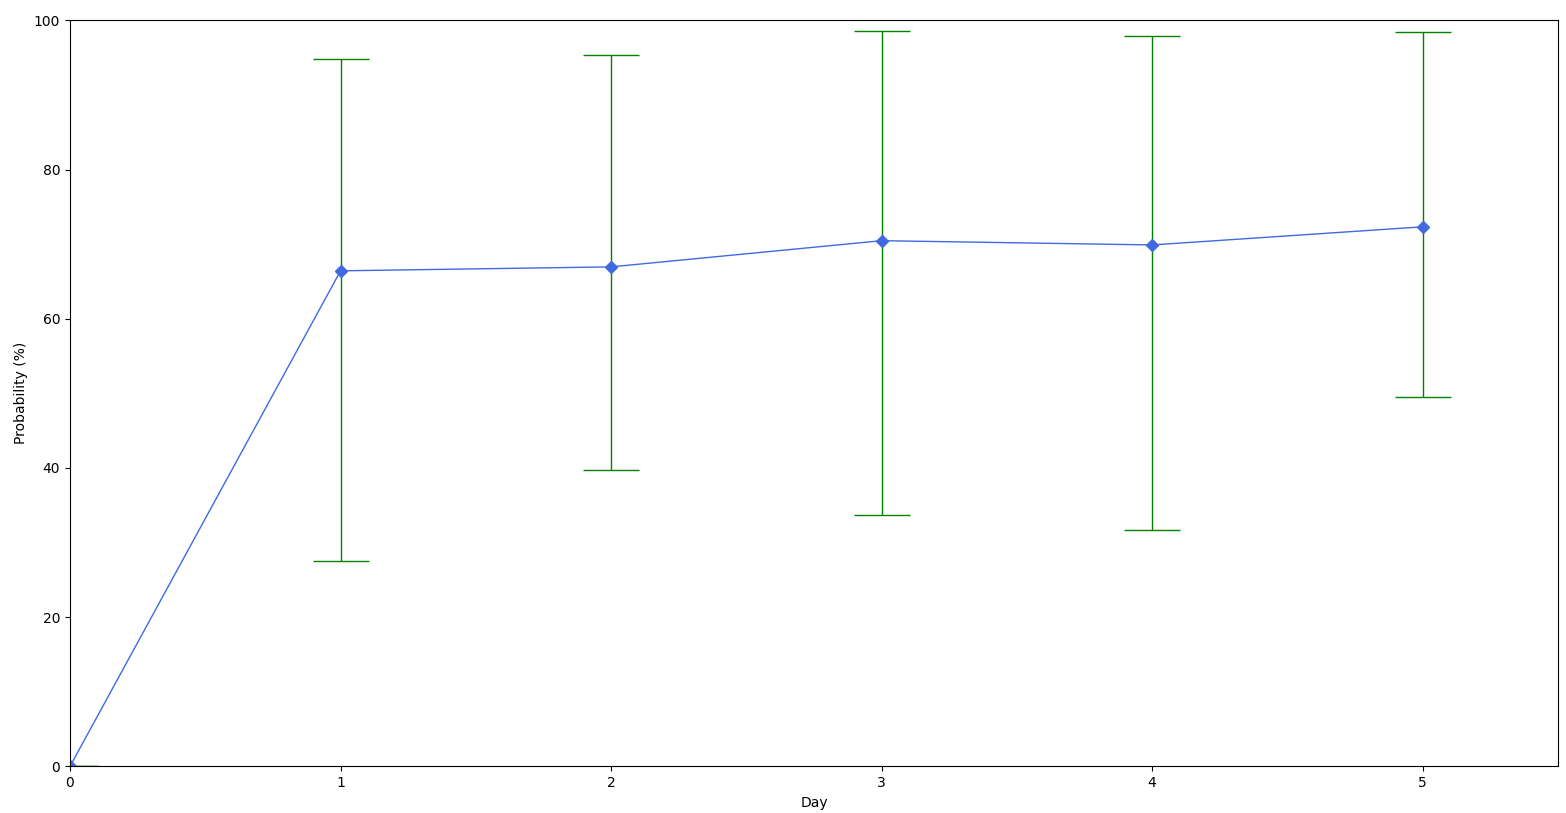
\includegraphics[scale=.4]{pic/acc_note.png}
      \caption[กราฟแสดงความแม่นยำเฉลี่ยของการระบุตัวตนของ 1 บุคคลในแต่ละวัน]{กราฟแสดงความแม่นยำเฉลี่ยของการระบุตัวตนของ 1 บุคคลในแต่ละวัน}
      \label{fig:face_graph}
    \end{center}
  \end{figure}

\indent ความแม่นยำเฉลี่ยของการระบุตัวตน 1 บุคคลในแต่ละวันคือ 66.42, 66.95, 70.46, 69.89 และ 72.32 เปอร์เซ็นต์ ตามลำดับ ความแม่นยำต่ำสุดของการระบุตัวตนในแต่ละวันคือ 27.4, 39.68, 33.65, 31.70 และ 49.51 เปอร์เซ็นต์ 
ตามลำดับ และความแม่นยำสูงสุดของการระบุตัวตนคือ 94.81, 95.38, 98.6, 97.94 และ 98.37 เปอร์เซ็นต์ ตามลำดับ

\subsection{ความแม่นยําของการระบุตัวตนด้วยใบหน้าในแต่ละวันของแบบจำลอง}
\begin{figure}[!ht]
    \begin{center}
      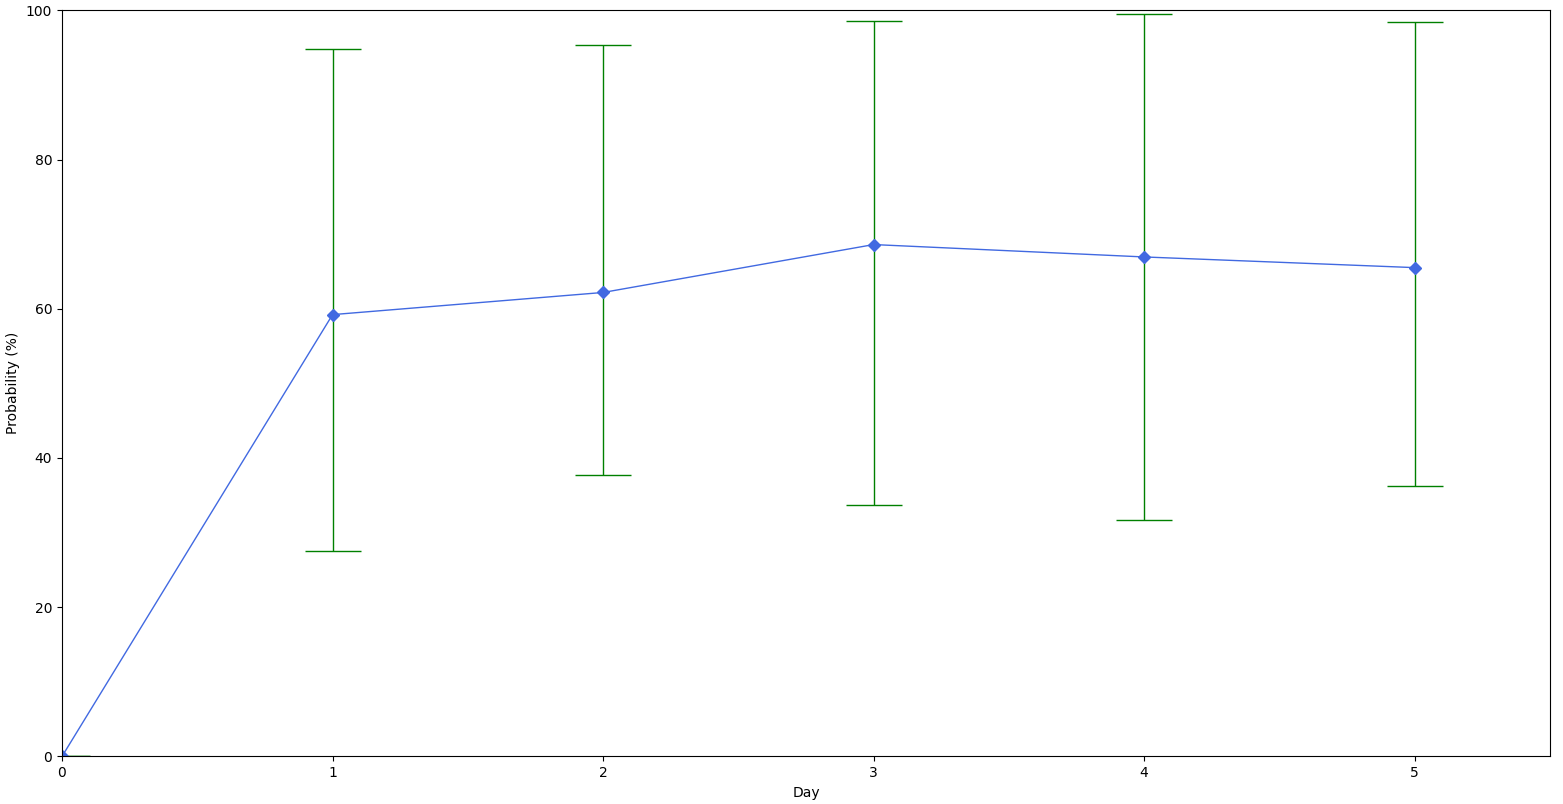
\includegraphics[scale=.4]{pic/acc_all.png}
      \caption[กราฟแสดงความแม่นยำเฉลี่ยของการระบุตัวตนของแบบจำลองในแต่ละวัน]{กราฟแสดงความแม่นยำเฉลี่ยของการระบุตัวตนของแบบจำลองในแต่ละวัน}
      \label{fig:face_graph_all}
    \end{center}
  \end{figure}


\indent ความแม่นยำเฉลี่ยของการระบุตัวตนจากแบบจำลองในวันที่ 1 คือ 59.21 เปอร์เซ็นต์ และในวันที่ 5 คือ 65.51 เปอร์เซ็นต์ จะเห็นว่าความแม่นยำของการระบุตัวตนเฉลี่ยเพิ่มขึ้น 6.3 เปอร์เซ็นต์ 
ซึ่งเป็นไปตามหลักการเรียนรู้ของเครื่องแบบต่อเนื่อง



\section{เวลาในการประมวลผลรูปภาพใบหน้า}
การทดสอบต่อไปนี้เป็นการทดสอบเพื่อวัดผลเวลาทั้งหมดของการประมวลผลรูปภาพใบหน้า ส่งรูปภาพไปยังเซิร์ฟเวอร์ ระบุตัวตน และการส่งผลลัพธ์กลับมาแสดงผลในหน้าจอ
โดยจะวัดเวลาในหน่วยของมิลลิวินาที (Millisecond) และบันทึกผลที่ Raspberry Pi โดยจะเปรียบเทียบเวลาที่วัดได้ในทุกครั้งที่มีการตรวจจับภาพใบหน้า 
ซึ่งจำนวนครั้งที่ตรวจจับใบหน้าบุคคลคือ 207 ครั้งจากทั้งหมด 5 วันที่ทำการทดลองแล้วสรุปผลออกมาเป็นกราฟ
  
\begin{figure}[!ht]
  \begin{center}
    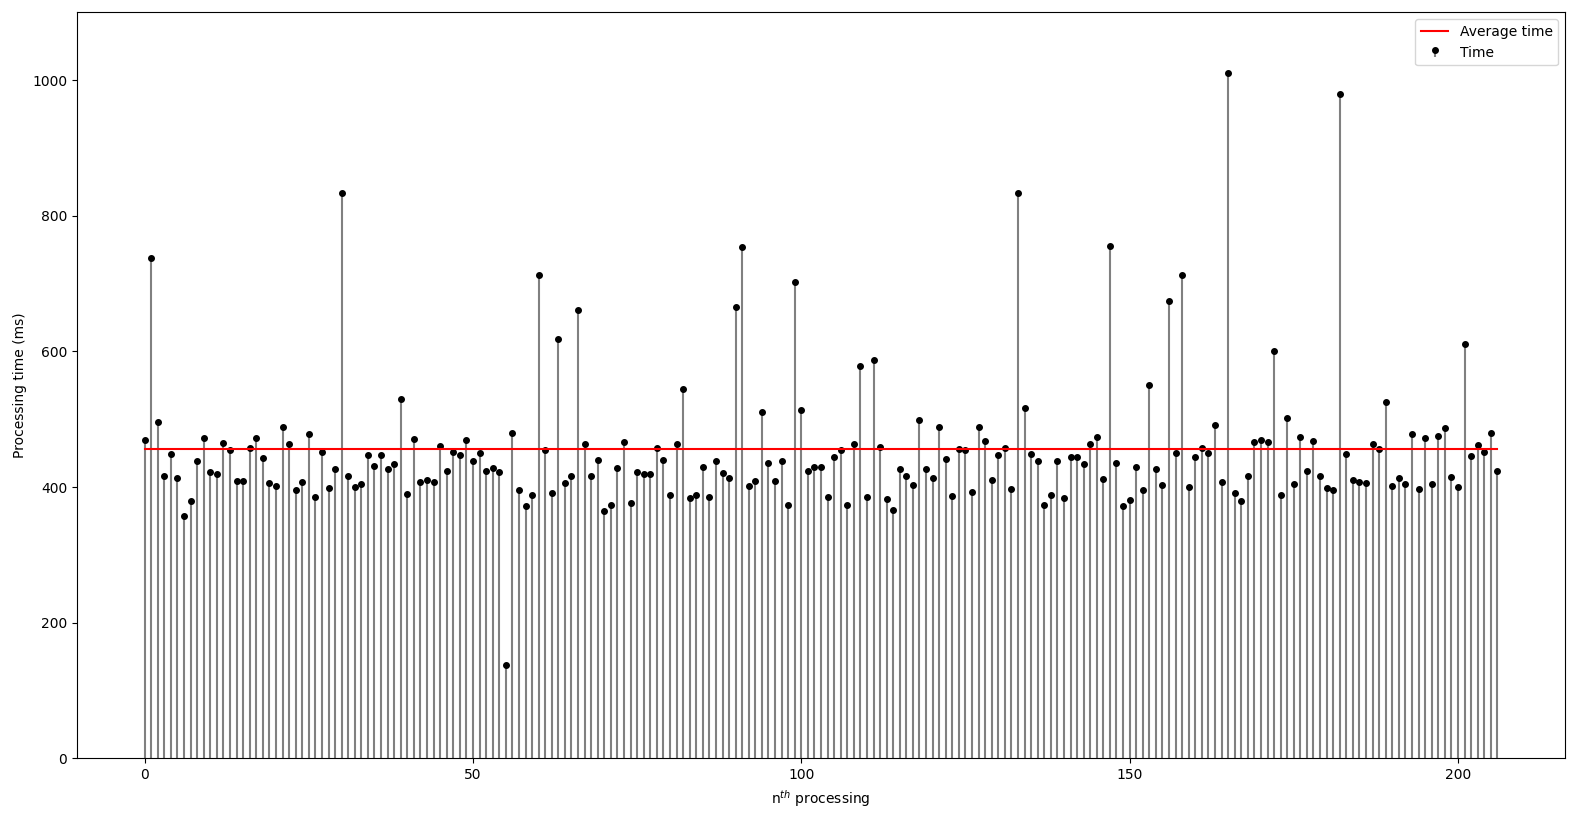
\includegraphics[scale=.4]{pic/Time_1.png}
    \caption[กราฟแสดงเวลาในการประมวลผลของระบบในแต่ละวัน]{กราฟแสดงเวลาในการประมวลผลของระบบในแต่ละวัน}
    \label{fig:time_graph}
  \end{center}
\end{figure}
\newpage
\indent จากกราฟจะเห็นได้ว่าเวลาในการประมวลผลรูปภาพใบหน้า ส่งรูปภาพไปยังเซิร์ฟเวอร์ การระบุตัวตน การส่งผลลัพธ์กลับมาแสดงผลในหน้าจอนั้นมีเวลาเฉลี่ย 455.62 มิลลิวินาที มากที่สุด 1010 มิลลิวินาที 
น้อยที่สุด 138 มิลลิวินาที และค่าเบี่ยงเบนมาตรฐานของเวลาในการประมวลผล คือ 99.19



\section{ความพึงพอใจของการทดลอง}
จากการทดลองที่ห้องวิจัย OASYS ได้ทำการบันทึกผลความพึงพอใจของผู้ทดลองต่อระบบระบุตัวตนด้วยรูปภาพใบหน้าบุคคล ในด้านต่าง ๆ ได้แก่ 
ความแม่นยำของการระบุตัวตน เวลาในการระบุตัวตน GUI แสดงผลการระบุตัวตน รูปร่างอุปกรณ์ให้คะแนนความถูกต้อง และการตอบสนองของ GUI โดยจะได้ผลสรุปดังนี้

\begin{figure}[!ht]
    \begin{center}
      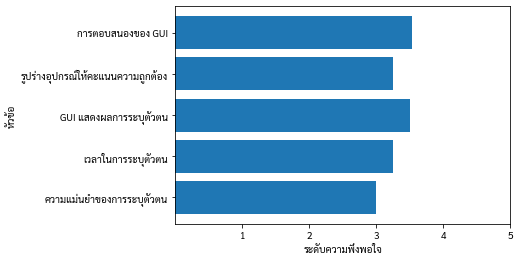
\includegraphics[scale=.6]{pic/test_graph.png}
      \caption[กราฟแสดงความพึงพอใจของผู้ทดลอง]{กราฟแสดงความพึงพอใจของผู้ทดลอง}
      \label{fig:bar_graph}
    \end{center}
  \end{figure}

\indent ผลความพึงพอใจของผู้ทดลองต่อระบบระบุตัวตนด้วยรูปภาพใบหน้าบุคคลในด้านความแม่นยำของการระบุตัวตนอยู่ที่ 3 (ปานกลาง) ในด้านเวลาในการระบุตัวตน GUI อยู่ที่ 3.25 (ปานกลาง)
ในด้านแสดงผลการระบุตัวตนอยู่ที่ 3.5 (ปานกลาง) ในด้านรูปร่างอุปกรณ์ให้คะแนนความถูกต้องอยู่ที่ 3.25 (ปานกลาง)  และในด้านการตอบสนองของ GUI อยู่ที่ 3.5 (ปานกลาง) 
และความคิดเห็นของผู้ใช้งานต่อระบบมีดังนี้
\begin{itemize}
  \item มีความแม่นยำมากกว่านี้ ควรระบุได้ว่าเราเป็นใคร
  \item ในขณะใช้งานระบบ พบว่าจะต้องยืนค้างเป็นระยะเวลาหนึ่ง ระบบจึงจะสามารถตรวจจับได้ หากจะนำไปใช้งานจริง ก็ควรจะพัฒนาให้การตรวจจับใบหน้าใช้เวลาที่น้อยลง 
\end{itemize}